\chapter{Gramática de Atributos Multi-planes (MAG)}
\label{chap:mag}
\minitoc

Tal como lo presenta Wuu-Yang en \cite{wuu-yang1} y como lo analizamos en la seccion \ref{XX}, la familia de \textit{gramática de atributos multi-planes} es una clase que se encuentra dentro de las WDAG y dentro de ellas de las NC.

La familia de las MAG es estrictamente mayor que las ANCAG. La importancia de esta familia radica en que el procedimiento de computación de planes de evaluación estáticos toma \textbf{tiempo polinomial} en el numero de símbolos y producciones.

A continuación trataremos en detalle la familia de las MAG y en el capítulo siguiente abordaremos el mecanismo de evaluación de las mismas.

% \section{Gramática de atributos}
% En esta sección, se define la notación que se usara en le desarrollo del presente capítulo para la definición de la familia MAG.
% Básicamente, la notación usada es la utilizada por Wuu yang en \cite{wuu-yang1}, la cual proviene de la notación de Kastens en \cite{kastens}.

\section{Preliminares}
\label{sec:pre-grafos}
Antes de llegar a la definición de la familia de \textit{gramáticas multi-plans}, presentaremos un ejemplo de gramática de atributos que servirá para estudiar conceptos previos, como lo son, la construcción de una serie de grafos necesarios para el análisis de los integrantes de dicha familia.

El ejemplo es presentado en la figura \ref{ag-no-ANCAG}. El mismo es trabajo, luego, en las etapas consideradas para el diseño de \maggen.

\begin{AG}

\newproduction{S}{XYZ}
    \begin{Attribution}
        \attribution{S.s0 := f(X.s1,Y.s2,Y.s3,Z.s4)}
        \attribution{X.i1 := Y.s3}
        \attribution{Y.i2 := X.s1}
        \attribution{Y.i3 := Y.s2}
    \end{Attribution}

\newproduction{Y}{m}    
    \begin{Attribution}
        \attribution{Y.s2 := Y.i2}
        \attribution{Y.s3 := 1}
    \end{Attribution}
    
\newproduction{Y}{n}
    \begin{Attribution}
        \attribution{Y.s2 := 2}
        \attribution{Y.s3 := Y.i3}
    \end{Attribution}
    
\newproduction{X}{m}
    \begin{Attribution}
        \attribution{X.s1 := X.i1}
    \end{Attribution}
    
\newproduction{Z}{Y}
    \begin{Attribution}
        \attribution{Z.s4 := Y.s3}
        \attribution{Y.i2 := 3}
        \attribution{Y.i3 := Y.s2}
    \end{Attribution}
\caption{Una gramática de atributos no ANCAG}
\label{ag-no-ANCAG}
\end{AG}
\subsection{Grafo \textit{DP}}
Los grafos \textit{DP} denotan las relaciones de dependencias directas entre las instancias de la gramática. 

Un grafo \textit{DP} esta definido (\cite{estruc-algorit}) con las siguientes consideraciones: 

\begin{itemize}
\item Los nodos denotan \textit{instancias} de una producción.
\item Las aristas denotan la dependencia entre las instancias. Una arista $X_{i}.a\rightarrow X{j}.b$, \footnote{con \textit{i} y \textit{j} índices de ocurrencias consistentes con alguna ecuación de la gramática} denota que la evaluación de la instancia \textit{$X_{i}.a$} depende de la evaluación de \textit{$Y_{i}.b$} 
\end{itemize}

El conjunto de dependencias directas de una producción, de la gramática, se denota como \textit{DP(p)}(\textit{p} producción de la gramática) y se define como:
\begin{definition}
Dada una producción p de una gramática de atributos definida como en \ref{def:grammarattr}, entonces
\begin{equation}
DP(p) = \{(X_{i}.a, X_{j}.b) | X_{i}.a \rightarrow Y_{j}.b \in R^{p} \}
\end{equation}
\end{definition}

La noción de dependencia directa y DP(p) fueron presentados, también, en el capítulo introductorio, cuando se presentó la definición de Árbol sintáctico atribuido (\label{def:ast-attr}).  
En la figura \ref{dp-wuu-yang} se observan los grafos DP para la gramática de la figura \ref{ag-no-ANCAG}.

\subsection{Grafo \textit{Down}}
Los grafos \textit{Down} denotan las relaciones de los atributos de un símbolo. 

Un grafo \textit{Down} esta definido (\cite{estruc-algorit}) con las siguientes consideraciones: 

\begin{itemize}
\item Los nodos denotan \textit{atributos} de un símbolo.
\item Las aristas denotan la dependencia entre los atributos de un símbolo. Dado los atributos $a$ y $b\in A(X)$ del símbolo $X\in VN$, una arista $a\rightarrow b$, denota que la evaluación del atributo \texttt{a} depende de la evaluación de \texttt{b}. 
\end{itemize}
El conjunto de dependencias entre los atributos de un símbolo se denota como  
\texttt{Down(X)}($X\in VN$ de una gramática G) y se define:
\begin{definition}
Dada un símbolo X de una gramática de atributos definida como en \ref{def:grammarattr}, entonces
\begin{equation}
Down(X) = \{(a,b) | a \rightarrow b \} con\ a,b \in A(X)
\end{equation}
\end{definition}
En la figura \ref{down-wuu-yang} se muestran los grafos Down(X) y Down(Y) para la gramática de la figura \ref{ag-no-ANCAG}.

\subsection{Grafo \textit{DCG}}

\textit{DCG} significa \textit{Downward Characteristic Graphs}, los mismos contienen las dependencias entre instancias de la gramática para una producción \textit{p}, teniendo en cuenta un símbolo en la gramática.
\begin{definition}
Dado q una producción de la forma $X_{0}\rightarrow \alpha_{0} X_{1} \alpha_{1} X_{2} \dots X_{k} \alpha_{k}$, el \textit{Downward Characteristic graph} of $X_{0}$ en los subárboles derivados vía la producción \textit{q}, denotado como $DCG_{X_{0}}(q)$, es un grafo donde: 
\begin{itemize}
\item Los nodos son atributos del símbolo $X_{0}$.
\item Una arista, $X.a \rightarrow X.b$, denota una dependencia (transitiva) de X.b sobre X.a en algún subárbol derivado desde $X_{0}$ vía \textit{q}.
\end{itemize}
\end{definition}
Tomemos el siguiente teorema presentado por Wuu-Yang en \cite{wuu-yang1}:
\begin{theorem}
$\bigcup\limits_{\textit{todo p}}{DCG_{X} (p) = Down (X)}$
\end{theorem}
\underline{Nota:} $DCG_{X}(p)$ contiene las dependencias, entre las instancias de la gramática, para el símbolo \texttt{X}, acotando el análisis para la producción \textit{p} y los posibles contextos inferiores.

En la sección \ref{XXX} se analiza el algoritmo para construir los grafos DCG.

\subsection{Grafo \textit{ADP}}
\label{mag:adpdef}

Las siglas \textit{ADP} significan \textit{Augmented Dependency graph}. El grafo \textit{ADP} esta definido por instancias de la gramática, en los nodos, y cada arista se define como: $X_{i}.a\rightarrow X{j}.b$, denota que la evaluación de la instancia \textit{$X_{i}.a$} depende de la evaluación de \textit{$Y_{i}.b$}.

El conjunto de dependencias aumentadas se denota como $ADP (q | p_{1}, p_{2}, \dots, p_{k})$ y se define:
\begin{definition}
Sea q una producción de la forma $X_{0}\rightarrow \alpha_{0} X_{1} \alpha_{1} X_{2} \dots X_{k} \alpha_{k}$. Sea $p_{i}$ una producción cuya parte izquierda es $X_{i}$ ($1\leqslant i \leqslant k$). 
\begin{equation}
ADP (q | p_{1}, p_{2}, \dots, p_{k}) = DP(q) \bigcup\limits_{k}^{i=1}{DGC_{X_{i}}} (p_{i})
\end{equation}
\end{definition}

A partir de la definición anterior surge la siguiente:
\begin{definition}
El conjunto de todas las posibles dependencias aumentadas para una producción q se define como:
\begin{equation}
SADP(q) = \bigcup\limits_{q\in P}{ADP (q | p_{1}, p_{2}, \dots, p_{k})} 
\end{equation}
\end{definition}

\begin{figure}\centering
 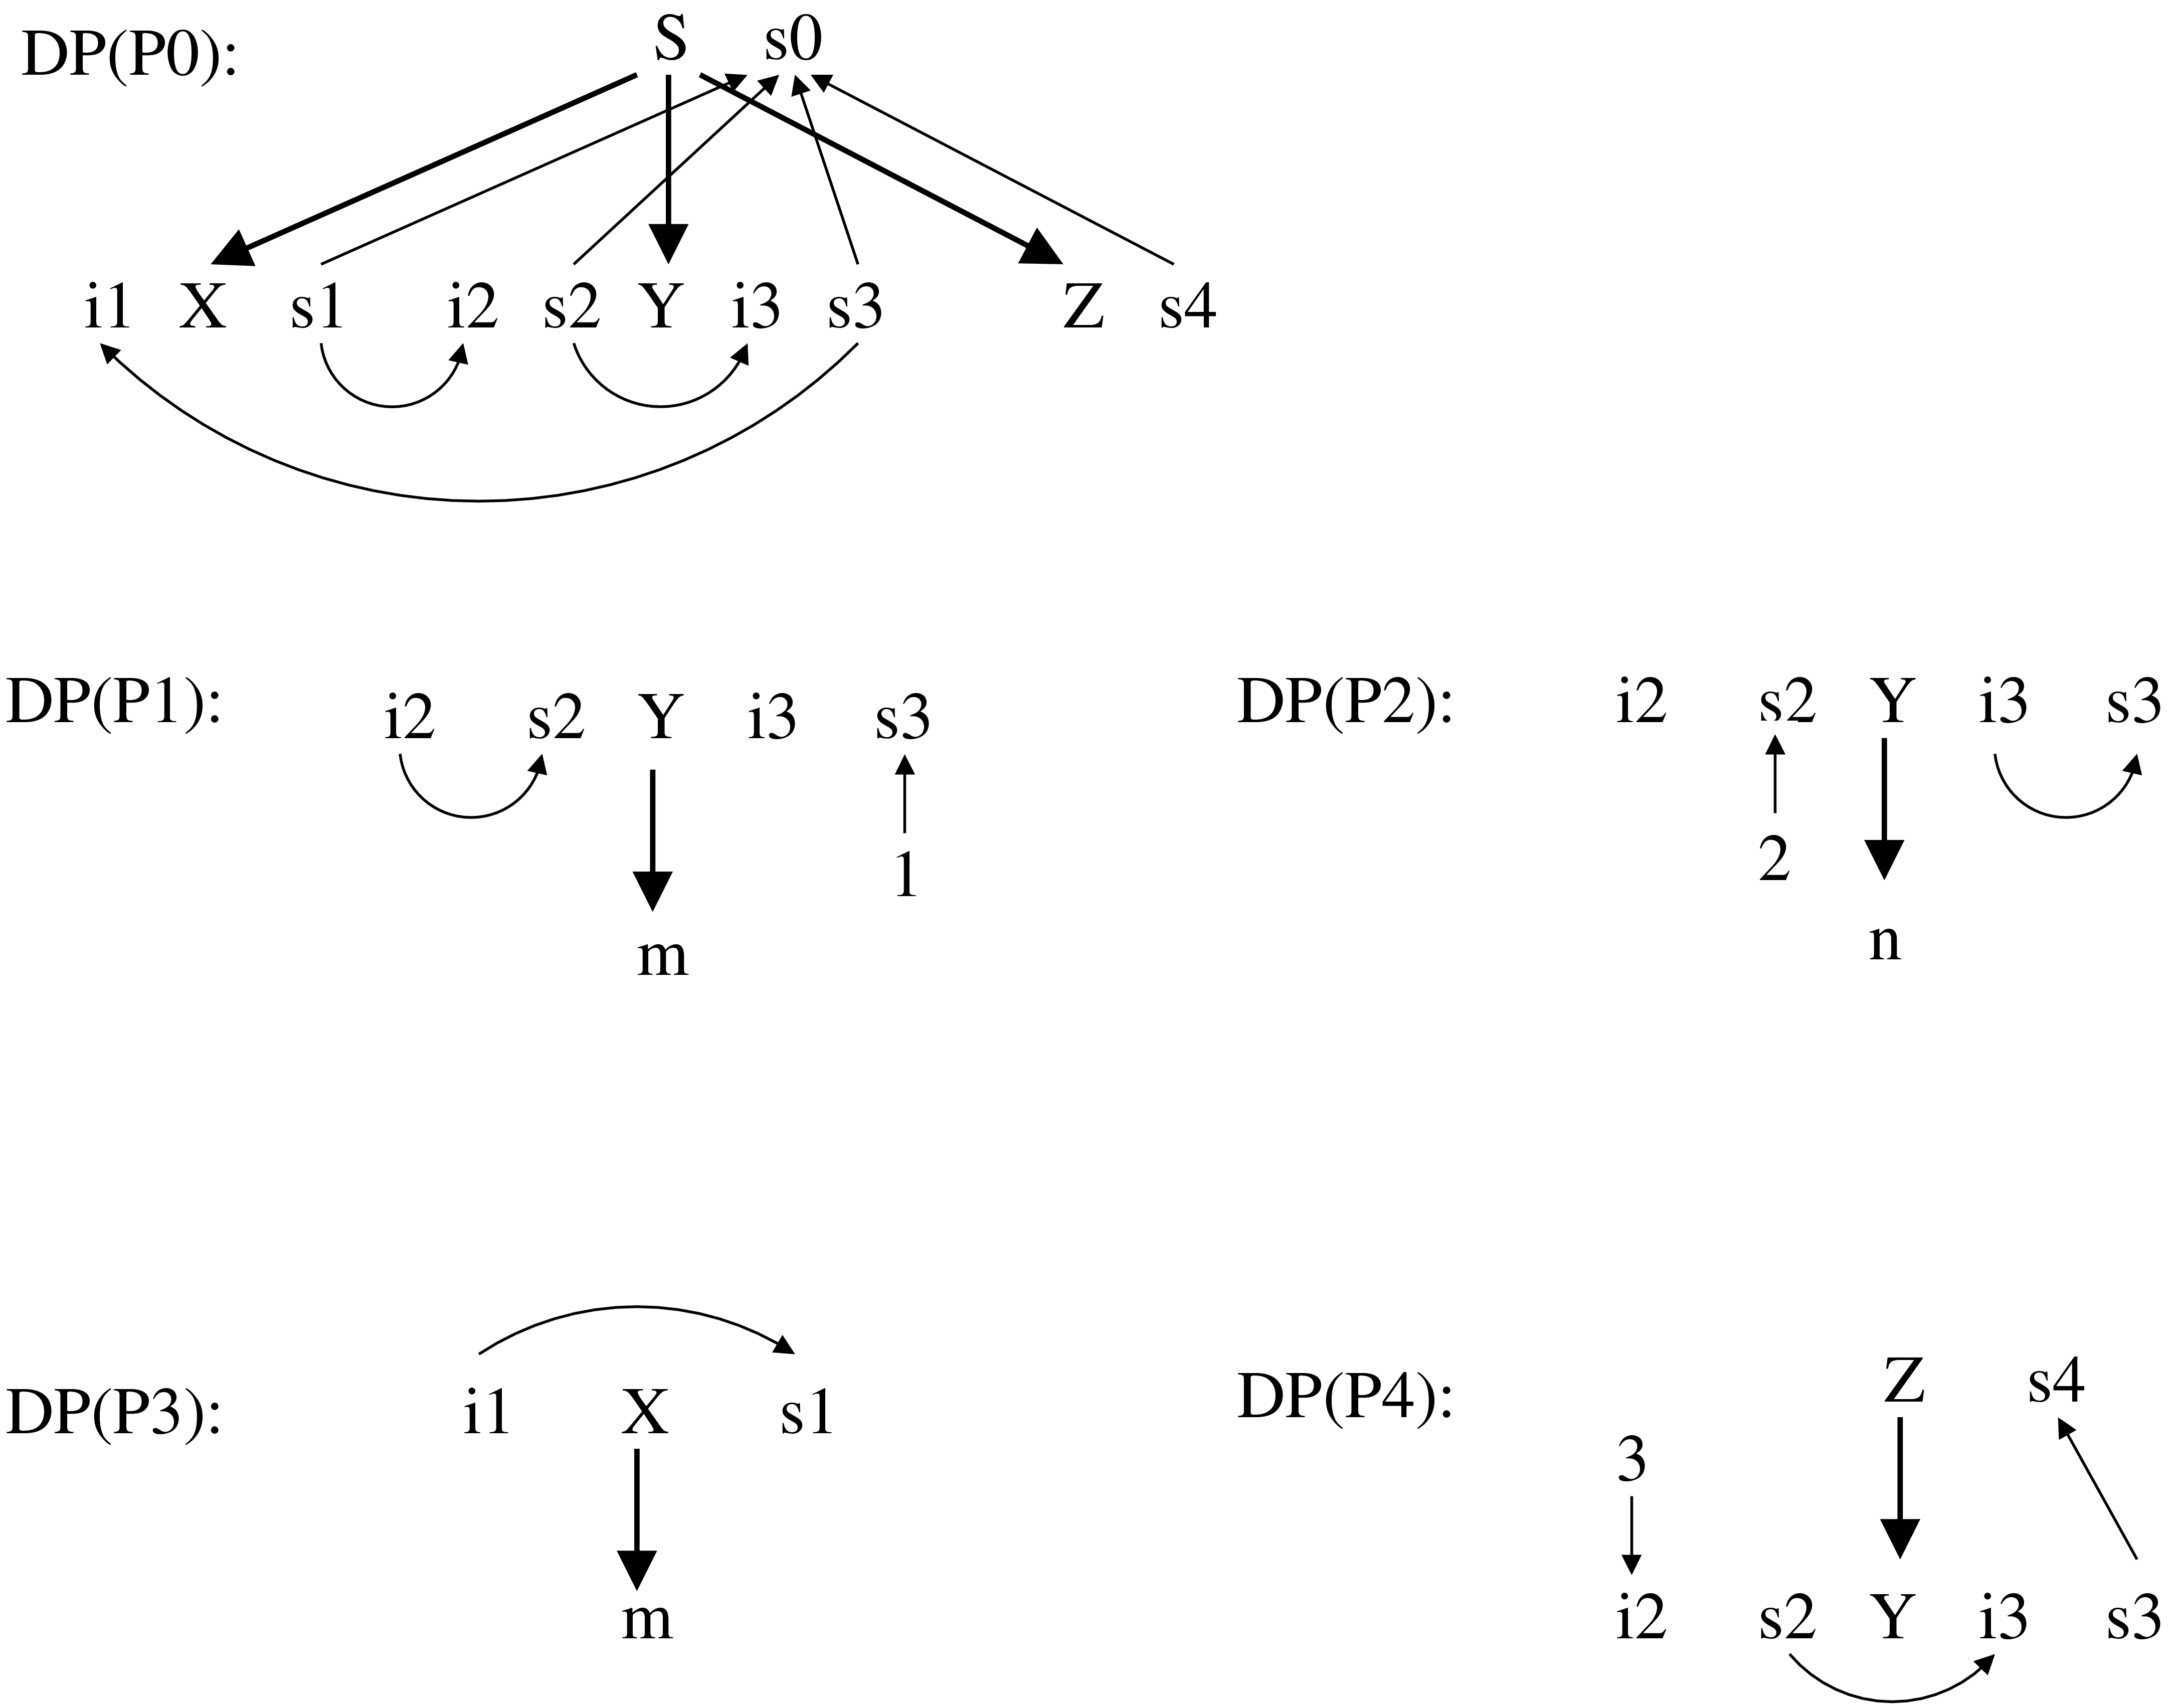
\includegraphics[width=250pt,height=195pt]{ej-grafos.png}
\caption{\label{dp-wuu-yang}Grafos DP para la gramática de la figura \ref{ag-no-ANCAG}.}
\end{figure}
\begin{figure}\centering
 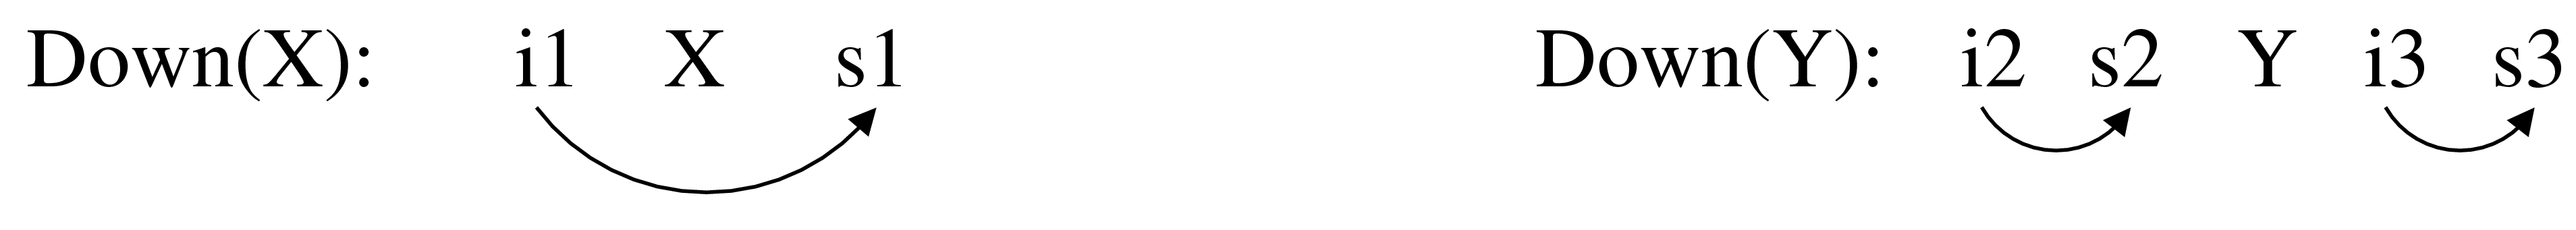
\includegraphics[width=350pt,height=31pt]{ej-grafos1.png}
\caption{\label{down-wuu-yang} DOWN(X) y DOWN(Y) para la gramática de la figura \ref{ag-no-ANCAG}.}
\end{figure}

\begin{figure}\centering
 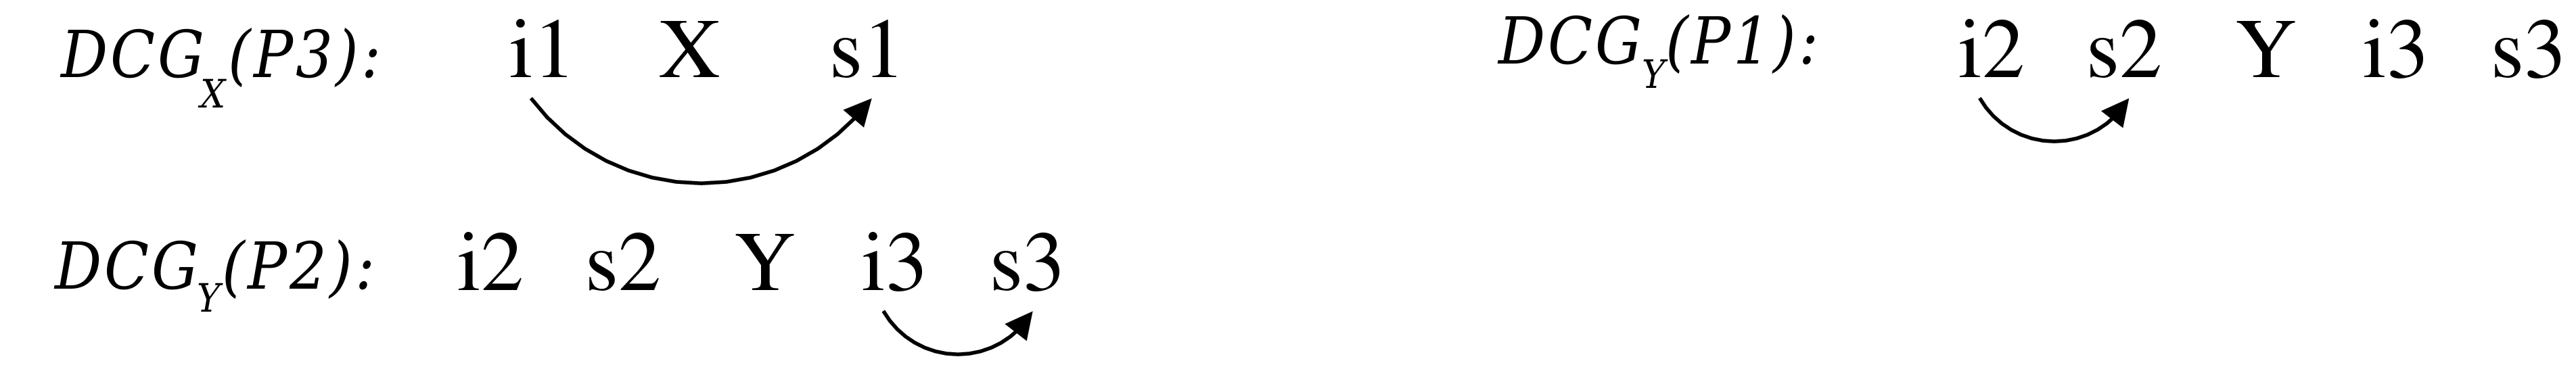
\includegraphics[width=350pt,height=52pt]{ej-grafos3.png}
\caption{\label{dcg-wuu-yang} Grafos DCG para la gramática de la figura \ref{ag-no-ANCAG}.}
\end{figure}

\begin{figure}\centering
 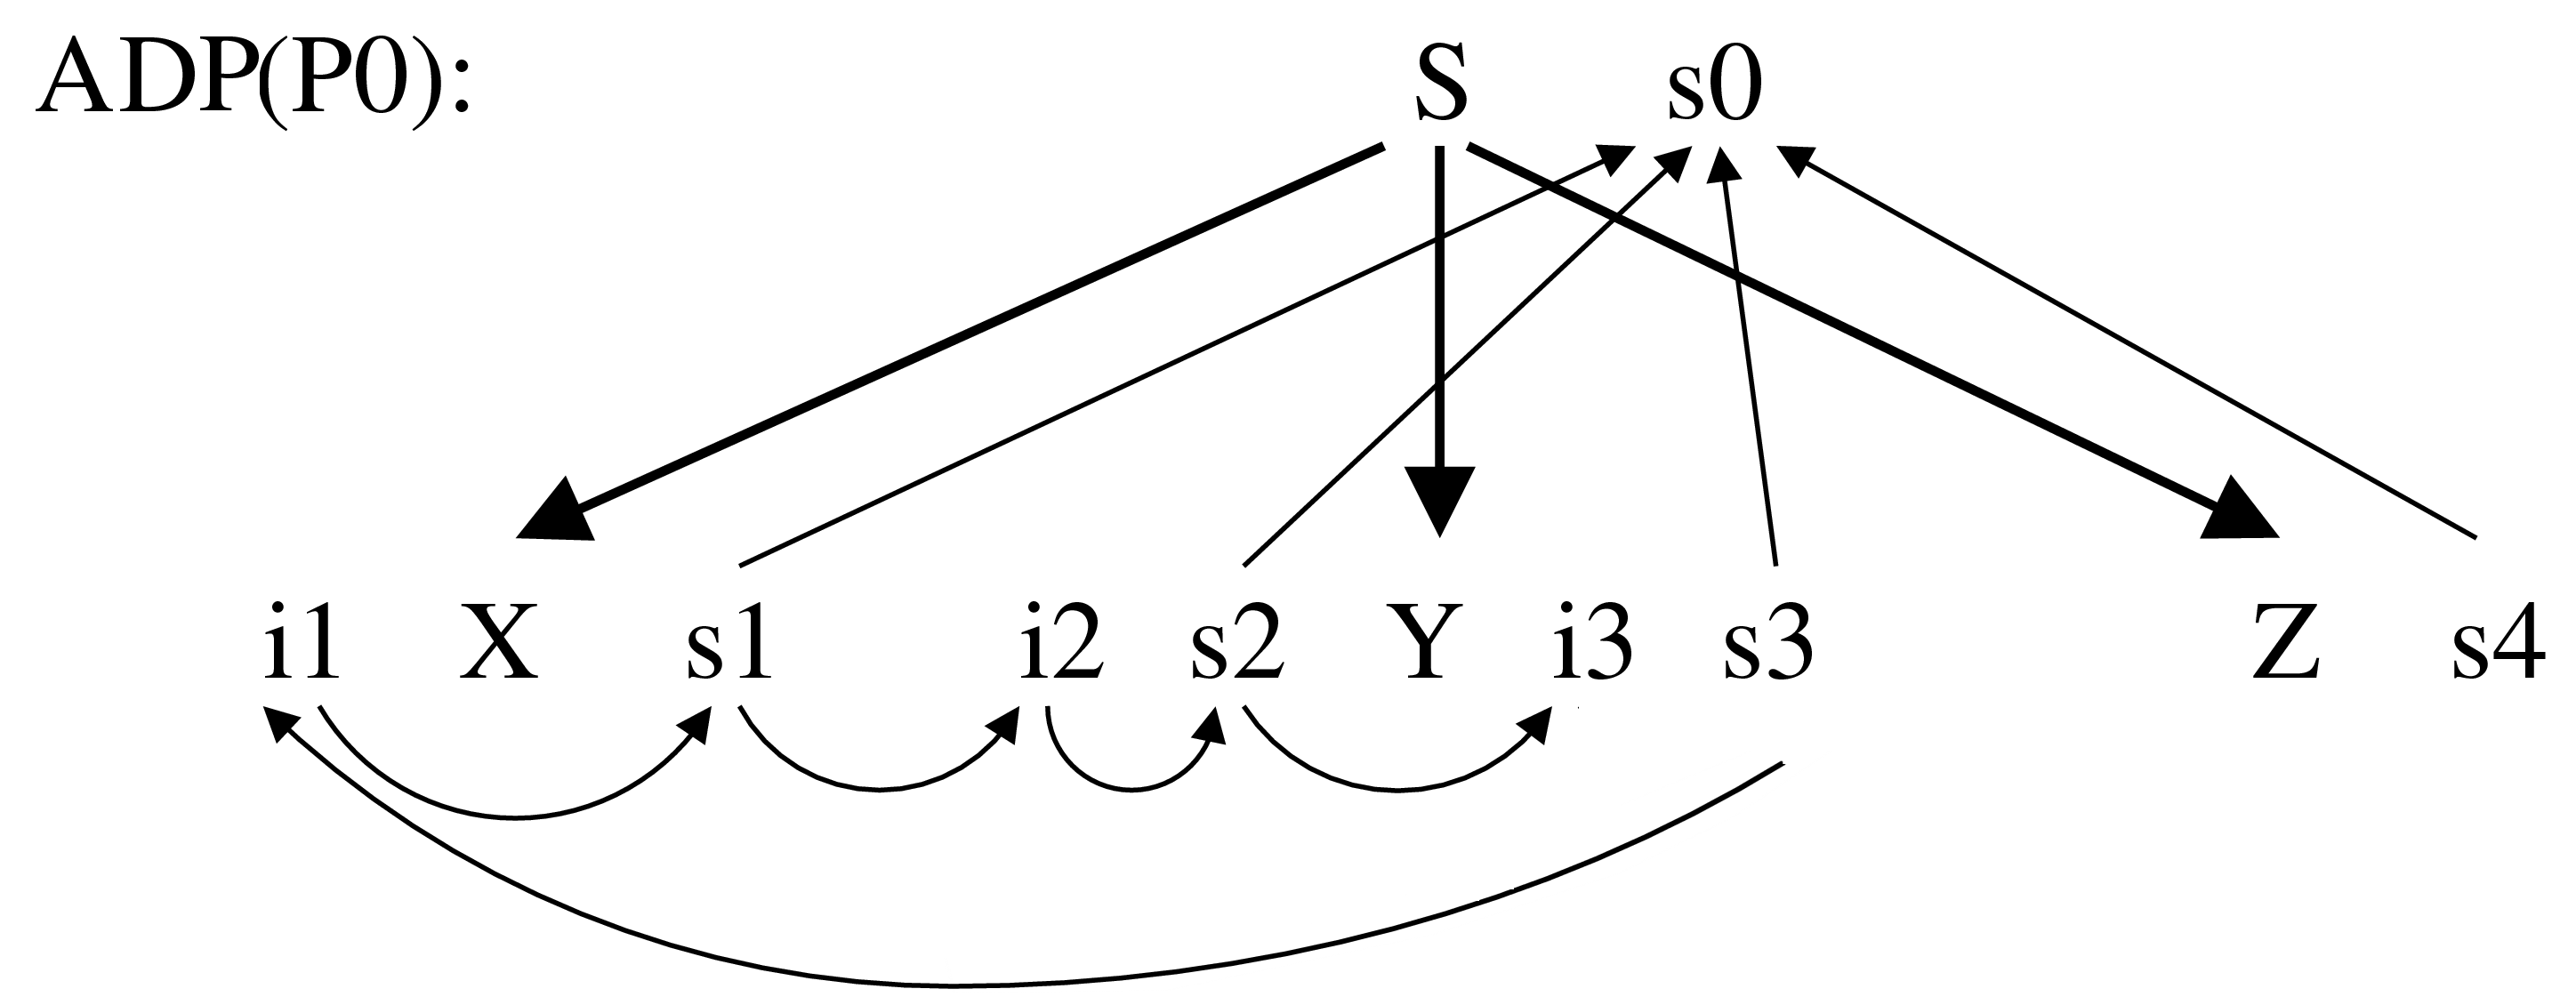
\includegraphics[width=350pt,height=132pt]{ej-grafos4.png}
\caption{\label{adp-wuu-yang} ADP(P0):contexto inferior P1, para la gramática de la figura \ref{ag-no-ANCAG}.}
\end{figure}

\section{Definición MAG}
\label{def:MAG}
Una gramática \textit{G} de la forma \ref{def:grammarattr} es una \textit{gramática de atributos multi-planes} si y solo si 
\begin{equation}
\forall q : q \in P: (\forall g:g\ es\ un\ grafo\ de\ q \wedge g \in SADP(q) : g\ es\ no\ circular) 
\end{equation}

Las \textit{gramáticas multi-plans} mantienen propiedades deseables como:
\begin{itemize}
\item La clases de gramáticas MAG cumplen la propiedad de que todas las gramáticas de atributos en dicha clase son \textbf{no circulares}.
\item Toda gramática MAG cumple con las propiedades de gramática bien definida\footnote{Es importante tener en cuenta las condiciones para gramática completa, detallada en \ref{def:gacompleta}} (WDAG), esto es, todo árbol sintáctico derivado sobre una MAG contiene dependencias no circulares.
\end{itemize}


De los conceptos analizado arriba surgen la siguiente definición y los siguientes 2 teoremas:

\begin{definition}
\label{def:ancag}
 Sea una \textit{q} una producción de la forma $X_{0}\rightarrow \alpha_{0} X_{1} \alpha_{1} X_{2} \dots X_{k} \alpha_{k}$ definimos:
\begin{equation}
 IDP-ANCAG(q) = DP(q) \bigcup\limits_{k}^{i=1}{Down(X_{i})}
\end{equation}

\end{definition}

\begin{theorem}
\label{th:ancag1}
$IDP-ANCAG(q) = \bigcup SADP(q)$, para toda producción q. 
\end{theorem}

\begin{theorem}
\label{th:ancag2}
Toda gramática ANCAG es una gramática MAG, pero no viceversa.
\end{theorem}

\begin{figure}\centering
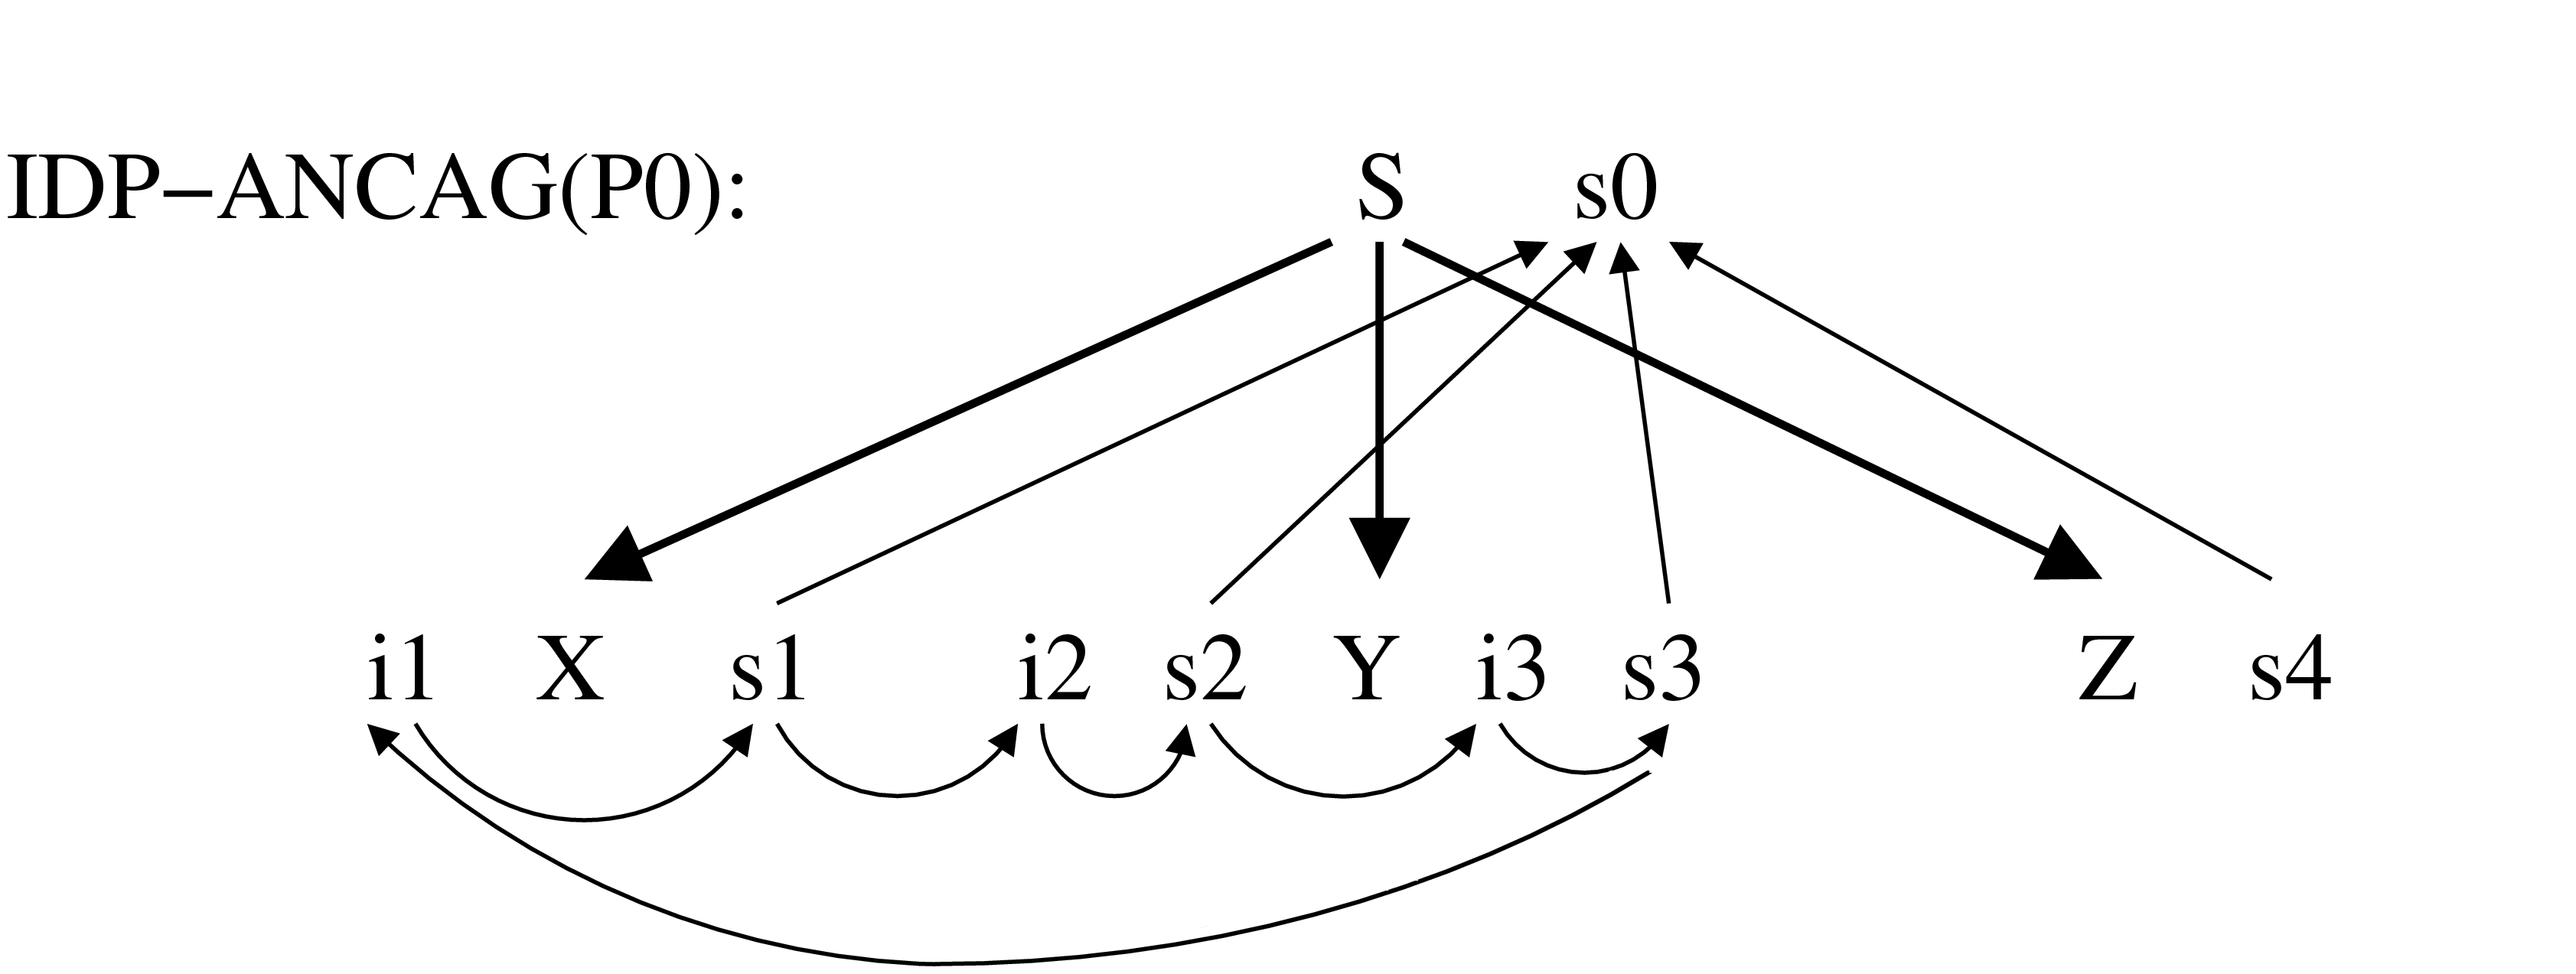
\includegraphics[width=350pt,height=132pt]{ej-grafos2.png}
\caption{\label{idp-wuu-yang}Grafo IDP-ANCAG(P0) para el ejemplo \ref{ag-no-ANCAG}.}
\end{figure}

Un resultado que muestra la veracidad del teorema anterior se observa en la gramática de la figura \ref{ag-no-ANCAG}, la cual es gramática MAG, pero la misma no es ANCAG. Este resultado se puede notar en la figura \ref{ancag-circle}, donde se marca la dependencia circular en el grafo.

\begin{figure}[t!]\centering
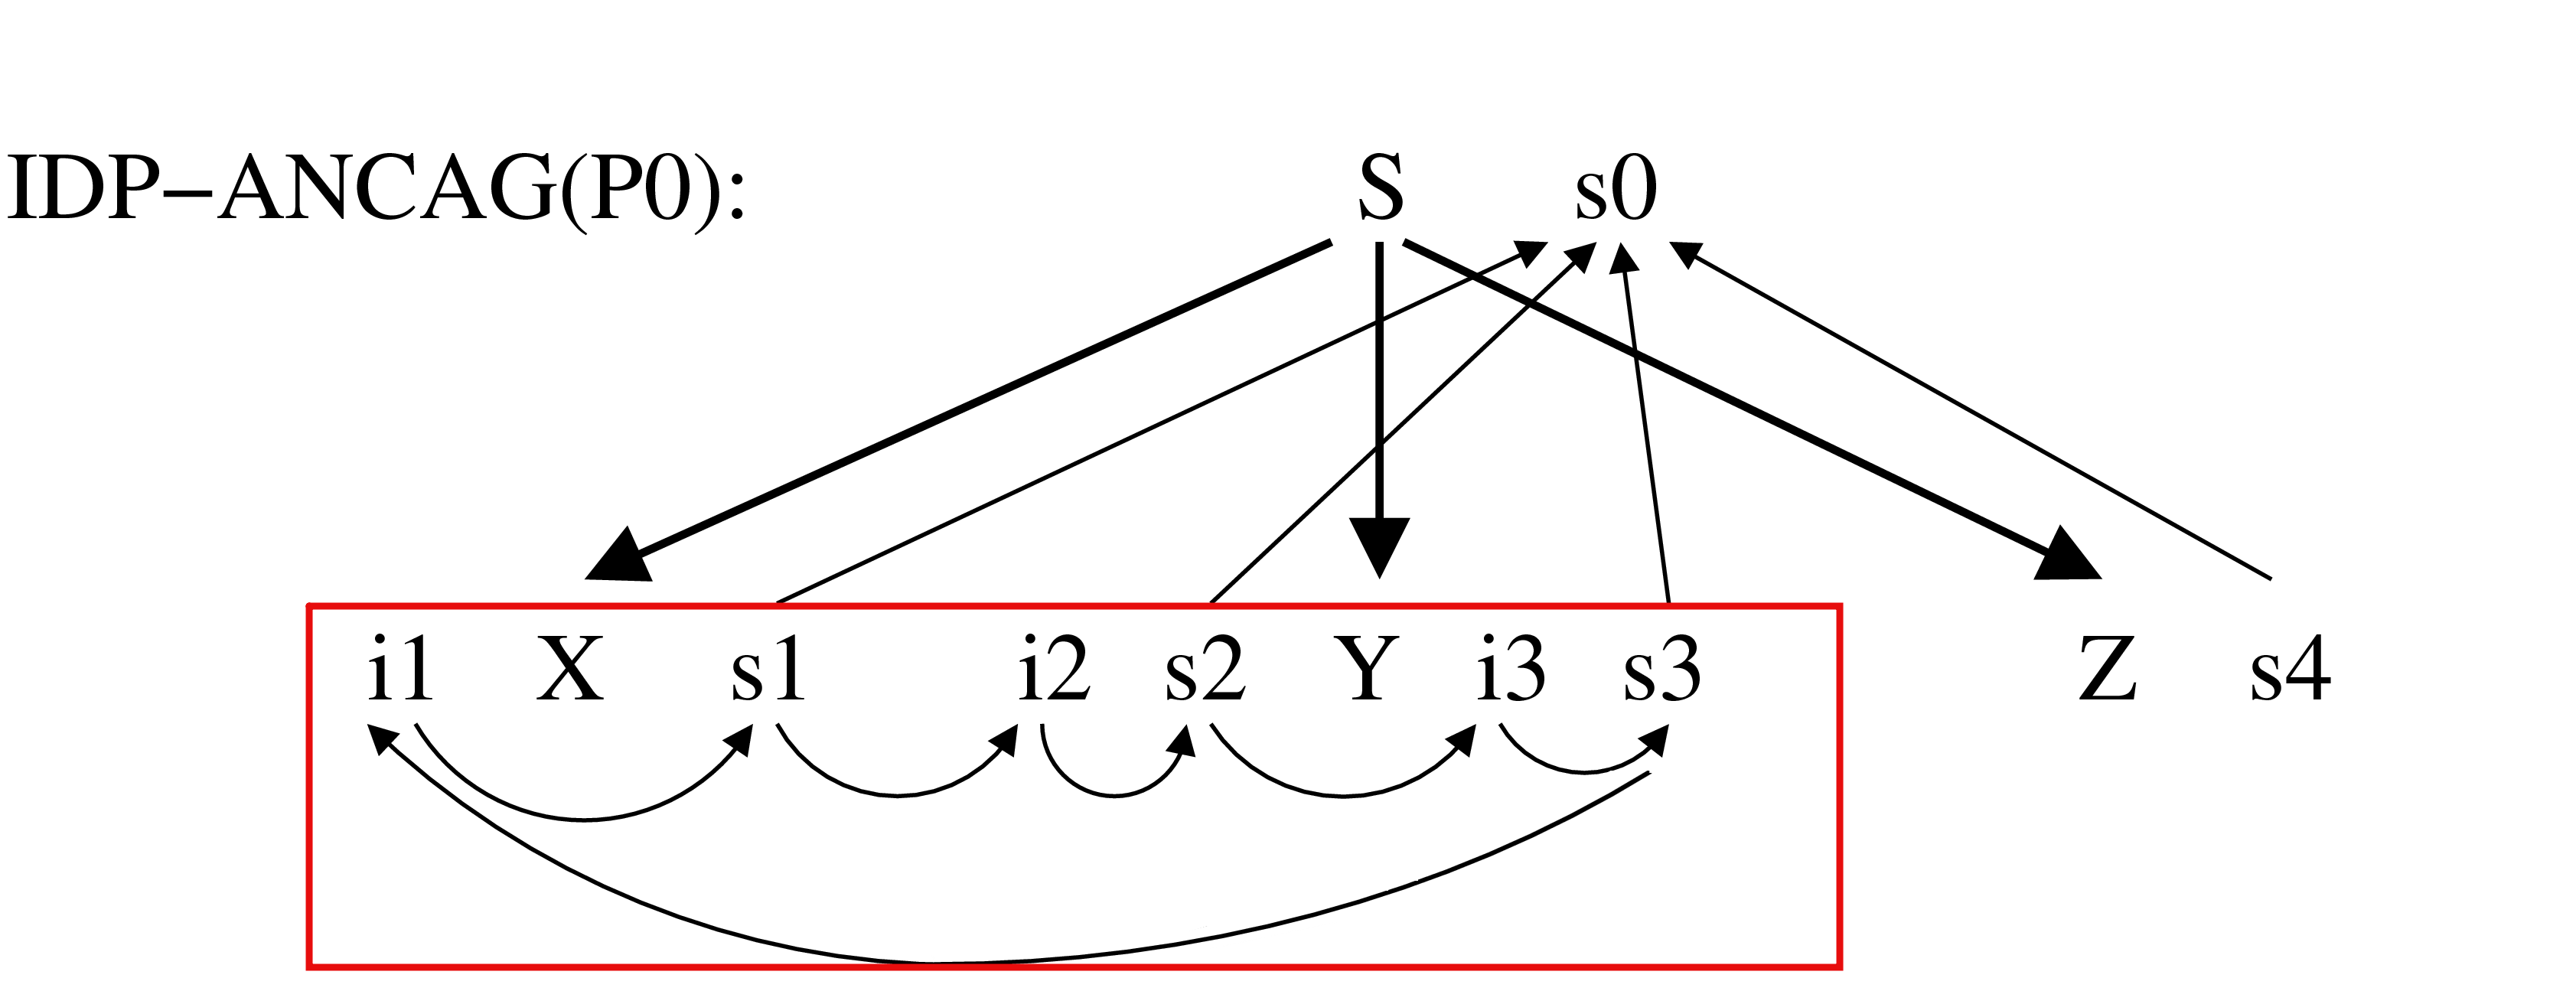
\includegraphics[width=350pt,height=135pt]{ej-grafos2-circle.png}
\caption{\label{ancag-circle} Grafo IDP-ANCAG(P0) marcando ciclo.}
\end{figure}
